\documentclass{beamer}

\usefonttheme{professionalfonts} % using non standard fonts for beamer
\usefonttheme{serif} % default family is serif

\usepackage{hyperref}
%\usepackage{minted}
\usepackage{animate}
\usepackage{graphicx}
\def\Put(#1,#2)#3{\leavevmode\makebox(0,0){\put(#1,#2){#3}}}
\usepackage{color}
\usepackage{tikz}
\usepackage{amssymb}
\usepackage{enumerate}


\newcommand\blfootnote[1]{%

  \begingroup

  \renewcommand\thefootnote{}\footnote{#1}%

  \addtocounter{footnote}{-1}%

  \endgroup

}

\makeatletter

%%%%%%%%%%%%%%%%%%%%%%%%%%%%%% Textclass specific LaTeX commands.

 % this default might be overridden by plain title style

 \newcommand\makebeamertitle{\frame{\maketitle}}%

 % (ERT) argument for the TOC

 \AtBeginDocument{%

   \let\origtableofcontents=\tableofcontents

   \def\tableofcontents{\@ifnextchar[{\origtableofcontents}{\gobbletableofcontents}}

   \def\gobbletableofcontents#1{\origtableofcontents}

 }

%%%%%%%%%%%%%%%%%%%%%%%%%%%%%% User specified LaTeX commands.

\usetheme{Malmoe}

% or ...

\useoutertheme{infolines}

\addtobeamertemplate{headline}{}{\vskip2pt}

\setbeamercovered{transparent}

% or whatever (possibly just delete it)

\makeatother

\begin{document}

\begin{frame}{Window operations}
    \centering
    \begin{figure}
        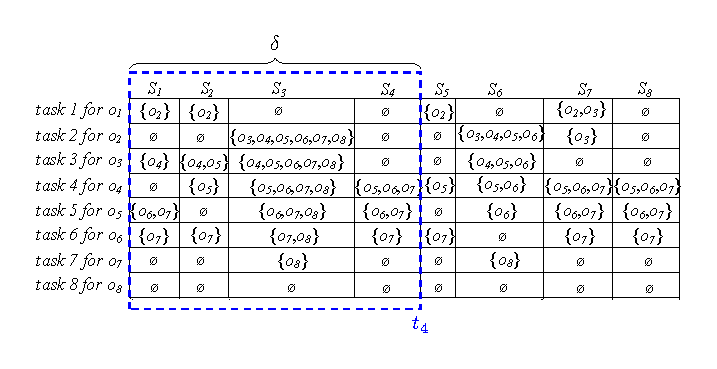
\includegraphics[width=.9\textwidth]{figures/Window01}
    \end{figure}    
\end{frame}
\begin{frame}{Window operations}
    \centering
    \begin{figure}
        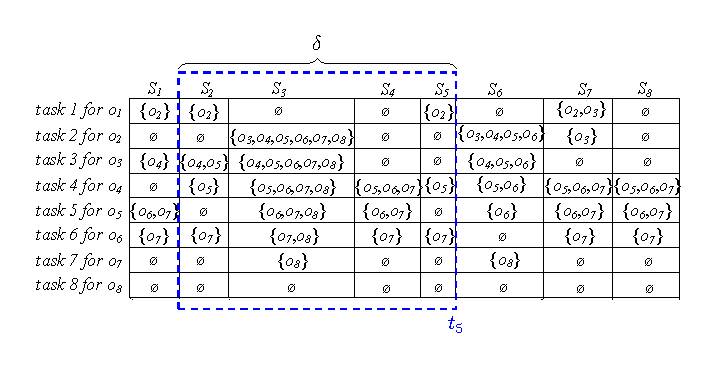
\includegraphics[width=.9\textwidth]{figures/Window02}
    \end{figure}    
\end{frame}
\begin{frame}{Window operations}
    \centering
    \begin{figure}
        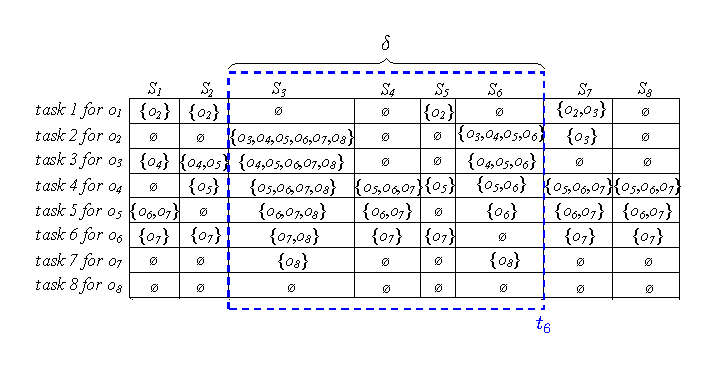
\includegraphics[width=.9\textwidth]{figures/Window03}
    \end{figure}    
\end{frame}
\begin{frame}{Window operations}
    \centering
    \begin{figure}
        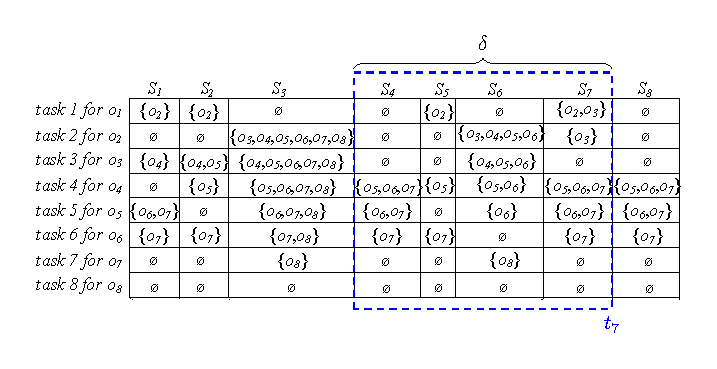
\includegraphics[width=.9\textwidth]{figures/Window04}
    \end{figure}    
\end{frame}
\begin{frame}{Window operations}
    \centering
    \begin{figure}
        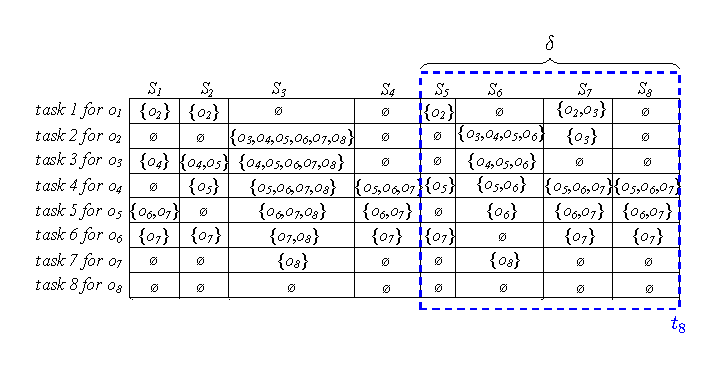
\includegraphics[width=.9\textwidth]{figures/Window05}
    \end{figure}    
\end{frame}

\end{document}
